% ============================================================
%  CHAPTER 6: ANDROID APPLICATION DESIGN AND USER INTERFACE
% ============================================================

\chapter{ANDROID APPLICATION DESIGN AND USER INTERFACE}
\label{chap:android_ui}

\section{Minimalist White Design Philosophy}
\label{sec:ui_design_philosophy}

The user interface of QuantumSafe VPN is engineered under a strict minimalist white design philosophy. In contemporary mobile application development, cybersecurity utilities frequently deploy visual bloat---dark glowing neons, aggressive 3D animations, and skeuomorphic dials that consume unnecessary CPU cycles, elevate battery drain, and obscure vital operational telemetry.

In contrast, QuantumSafe VPN embraces a clean technical aesthetic inspired by precision laboratory instruments, Swiss graphic typography, and Google's Material 3 guidelines:
\begin{itemize}
    \item Cognitive Efficiency: Critical network parameters (connection state, assigned virtual IP, tunnel duration, active cryptographic algorithms) are presented with immediate visual legibility.
    \item Restraint and Purpose: Every pixel serves a functional purpose. Shadows and purely decorative embellishments are replaced by clean structural 1\,dp borders and clear typography.
    \item Technical Transparency: The user interface treats the operator as an informed user, providing honest disclosure of cryptographic parameters, packet counters, and diagnostic logs rather than abstracting away the security mechanics.
\end{itemize}

Figure~\ref{fig:ui_screens_mockup} displays the four core screens comprising the QuantumSafe VPN Android client interface.

\begin{figure}[!t]
  \centering
  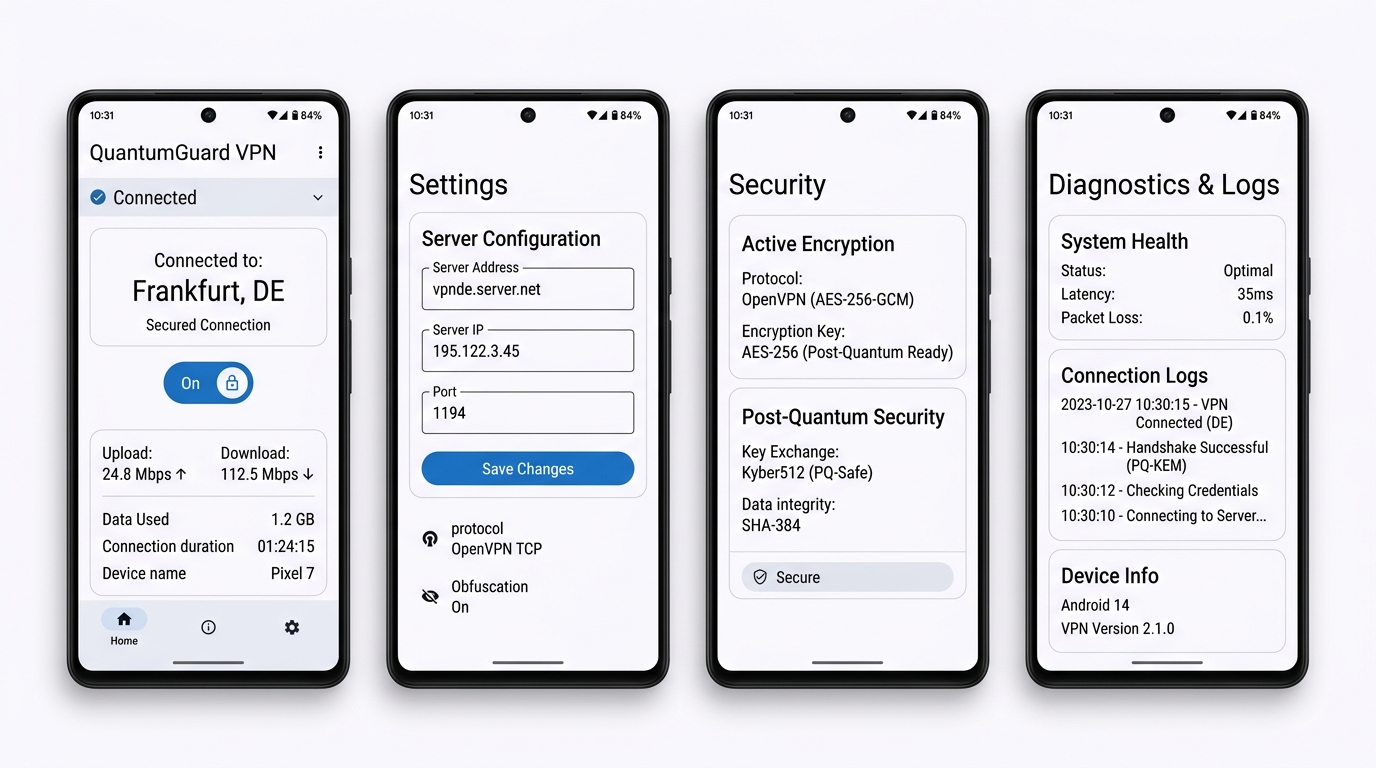
\includegraphics[width=0.82\linewidth,height=0.20\textheight,keepaspectratio]{figures/ui_screens_overview.jpg}
  \caption[Four-Screen Minimal White Design System Showcase]{Four-Screen Minimal White Design System Showcase of QuantumSafe VPN.}
  \label{fig:ui_screens_mockup}
\end{figure}

\section{Design System Tokens: Colors, Typography, and Metrics}
\label{sec:ui_design_tokens}

To enforce design consistency across the Kotlin Jetpack Compose codebase, the application implements a centralized token system within \texttt{ui/theme/Theme.kt} (Table~\ref{tab:design_tokens_color}).

\begin{table}[htbp]
  \centering
  \scriptsize
  \setlength{\tabcolsep}{3pt}
  \caption{Design System Tokens: Color Palette and Semantic Usage.}
  \label{tab:design_tokens_color}
  \begin{tabularx}{\linewidth}{@{}p{2.8cm}p{1.4cm}p{1.8cm}Y@{}}
    \toprule
    \textbf{Design Token} & \textbf{Hex} & \textbf{Visual} & \textbf{Semantic Application} \\
    \midrule
    Surface Pure White & \texttt{\#FFFFFF} & Pure White & Primary background surface for all screens and cards \\
    Surface Container & \texttt{\#F8F9FA} & Ultra-Light Gray & Contrast surface for nested telemetry containers \\
    Border Structural & \texttt{\#DEE2E6} & Light Neutral & 1\,dp structural dividers and card outlines \\
    Text High Contrast & \texttt{\#1A1D20} & Dark Charcoal & Primary typography, titles, and status headlines \\
    Text Secondary & \texttt{\#6C757D} & Medium Gray & Metadata labels, subtitles, and unit indicators \\
    Brand Primary Blue & \texttt{\#1971C2} & Marine Blue & Primary interactive button (Connect), active tabs \\
    Brand Accent Light & \texttt{\#E7F5FF} & Ice Blue Tint & Status badge container for active connection \\
    Status Success Green & \texttt{\#2B8A3E} & Forest Green & Connected state indicator dot and success alerts \\
    Status Warning Amber & \texttt{\#E67700} & Deep Amber & Connecting / handshaking in-progress indicator \\
    Status Error Red & \texttt{\#C92A2A} & Crimson Red & Disconnection alerts, handshake failure badges \\
    \bottomrule
  \end{tabularx}
\end{table}

\subsection{Typography and Spatial Metrics}
The typography scale leverages Google's Inter for headings and UI controls, paired with Roboto Mono for cryptographic hashes, IP addresses, and diagnostic logs. Spatial layout adheres to an 8-point grid: 16\,dp horizontal screen padding, 12\,dp component spacing, 12\,dp card corner radii, and 56\,dp primary button height with 0\,dp elevation shadows.

\section{Information Architecture and Screen Specifications}
\label{sec:screen_specifications}

The mobile client deploys a single-activity architecture (\texttt{MainActivity.kt}) hosting a top-level Scaffold with a minimal bottom navigation bar linking four dedicated views:

\subsection{Screen A: Home Screen (Primary Operational Dashboard)}
The Home screen serves as the core user surface:
\begin{enumerate}
    \item Status Badge Banner: Renders an interactive pill-shaped badge displaying operational state (e.g., \texttt{DISCONNECTED}, \texttt{CONNECTING}, \texttt{PROTECTED}, or \texttt{FAILED}).
    \item Session Telemetry: When active, displays a high-contrast monospace timer (\texttt{00:14:22}) alongside remote gateway endpoint (\texttt{11.12.5.8:7000}) and assigned virtual IP (\texttt{10.8.0.2}).
    \item Primary Action Control: A 56\,dp high button executing reactive state transitions (Brand Blue ``CONNECT'', disabled pulsing ``ESTABLISHING TUNNEL...'', and White/Crimson outline ``DISCONNECT'').
    \item Real-Time Throughput Cards: Twin white cards reporting live uplink/downlink rates (e.g., \texttt{24.8\,Mbps $\uparrow$}, \texttt{112.5\,Mbps $\downarrow$}) and cumulative data transfer volumes.
\end{enumerate}

\subsection{Screen B: Server Configuration Screen}
Allows network administrators to configure custom gateway endpoints via Material 3 outlined text fields with real-time regex validation: Server Hostname/IPv4, Port (default 7000), MTU (default 1400 bytes, range 1280--1500), and Socket Timeout. Configurations are securely persisted to the hardware-backed \texttt{SecurityManager} using AES-256-GCM.

\subsection{Screen C: Cryptographic Security Information Screen}
Provides total cryptographic transparency across four structured informational cards:
\begin{enumerate}
    \item Post-Quantum Key Exchange: ML-KEM-1024 (NIST FIPS 203), Category 5 ($\ge 256$-bit quantum margin), 1,568-byte public key and ciphertext.
    \item Identity Authentication: ML-DSA-65 (NIST FIPS 204), 1,952-byte public key, 3,309-byte signature, verified server identity pinning.
    \item Payload AEAD: AES-256-GCM (NIST SP 800-38D), HKDF-SHA256 with Keccak SHA3-256 derivation, 12-byte random IV, 16-byte Galois MAC tag.
    \item Anti-Replay Defense: 64-bit monotonic sequence counter with strict chronological admission.
\end{enumerate}

\subsection{Screen D: Diagnostics and Settings Screen}
Provides operational toggles (Auto-Reconnect, System Kill-Switch) and a live diagnostic terminal displaying events emitted by \texttt{VpnService}\allowbreak\texttt{Bridge}. Diagnostic actions include one-tap Ping Verification, DNS Leak Testing, and log export.

\section{Accessibility and Reactive Compose Mechanics}
\label{sec:accessibility_compose}

Accessibility compliance satisfies WCAG 2.1 AAA: dark charcoal text (\texttt{\#1A1D20}) against pure white (\texttt{\#FFFFFF}) provides a contrast ratio of 16.8:1 (well above the 7:1 AAA standard); all touch targets enforce a minimum of $48 \times 48$\,dp; and every composable specifies semantic \texttt{contentDescription} attributes for TalkBack screen readers.

The UI architecture enforces Unidirectional Data Flow (UDF) through a dedicated ViewModel. UI composables observe state reactively, ensuring that background networking events trigger granular, thread-safe recompositions without UI jank, maintaining a smooth 60\,fps interface.
